\begin{comment}
\end{comment}

\chapter{Circuits pour la tolérance aux fautes quantique}

Pour terminer le récit de ma thèse,
j'ajoute un niveau de réalisme au modèle de correction d'erreurs quantique
du chapitre précédent pour présenter la conception d'une mémoire quantique.
Une mémoire quantique est un système quantique permettant de stocker
de l'information pour une durée indéterminée.
Cependant,
tel que mentionné au chapitre précédent,
les systèmes quantiques sont sujets aux erreurs,
même lorsque aucune opération n'est effectuée.
Ainsi,
pour construire une mémoire quantique,
il est nécessaire, encore une fois,
d'utiliser un code correcteur pour corriger les erreurs au fur et à mesure
qu'elles affectent le système.
Du moins,
il faut s'assurer que les erreurs restent assez faibles afin de pouvoir utiliser
l'information stockée dans le système pour un calcul futur.

En principe,
il est possible d'utiliser n'importe quel code correcteur pour construire
une mémoire quantique,
mais certains ont des propriétées plus favorables.
D'abord,
il est difficile de mettre à l'échelle un code correcteur dont le graphe
de Tanner est local, soit un graphe où la distance entre chaque paire de sommets 
connectés par une arête est bornée indépendemment du nombre de sommets.
Plus précisément,
Bravyi, Poulin et Terhal~\cite{bravyi_tradeoffs_2010}
ont montré que pour un tel code $[n, k]$,
la distance minimale $d$ est limitée par
\begin{equation}
	d^2 \leq c \frac{n}{k},
\end{equation}
pour une constante $c$ indépendente de $n$, $k$ et $d$.
Ainsi,
si $k$ augmente proportionnellement avec $n$,
la distance minimale est bornée par une constante.
De plus,
pour avoir une distance minimale raisonnable,
il est nécessaire que le nombre de qubits encodés $k$ 
n'augmente pas ou très peu avec $n$.

Ce résultat implique que pour un grand $n$,
soit peu de qubits sont encodés,
soit ces derniers sont mal protégés des erreurs.
Il est donc difficile d'utiliser ces codes pour construire une mémoire 
quantique de grande taille.
Cependant,
lorsque la contrainte de localité du graphe de Tanner est abandonnée,
Gottesman~\cite{gottesman_fault-tolerant_2013} a montré qu'il est possible 
de construire une mémoire quantique protégeant efficacement les erreurs,
avec $\frac{k}{n}$ constant, en utilisant des codes LDPC.
Conséquemment,
il est possible d'utiliser des codes LDPC pour construire 
des mémoires quantiques de grandes échelles.

D'un point de vue expérimentale,
les codes LDPC ont l'avantages de pouvoir être implémentés de sorte que 
chaque qubit soit connecté à un nombre bornée d'autres qubits.
Comme je le présenterai plus tard lorsque j'introduirai les circuits
de mesures de syndromes,
cela permet d'implémenter efficacement les circuits nécessaires à la
construction d'une mémoire quantique,
à la condition de pouvoir coupler n'importe quelle paire de qubits 
indépendemment de la distance qui les sépare.

Comme les couplages à long portée sont difficiles pour plusieurs technologie de qubits,
il est tentant d'essayer d'implémenter des codes dont le graphe de Tanner est non local
à l'aide d'une architecture de qubits intéragissant localement,
quite à payer un léger surcout.
Cependant,
dans un article qui n'est pas présenté dans cette thèse~\cite{delfosse_bounds_2021},
Nicolas Delfosse, Michael Beverland et moi-même avons montré que le cout de cette approche
est en réalité beaucoup trop élevé.
Plus précisément,
nous avons montré que pour implémenter une mémoire à l'aide d'un bon code LDPC
avec un rendement $k/n$ constant,
le nombre total de qubits nécessaires $N$ et la profondeur du circuit $\tau$ sont 
bornée inférieurement par 
\begin{align}
	N^{1/2} \tau \geq c n,
\end{align}
où $c$ est une constante.
Ainsi,
soit un très grand nombre de qubits sont nécessaires,
soit le circuit doit être très long.
Dans les deux cas,
augmenter ces quantités offre plus d'occasions aux erreurs de ce manifester,
ce qui réduit significativement la qualité de la mémoire.

L'article présenté dans ce chapitre introduit une nouvelle architecture pour une mémoire quantique
qui permet d'implémenter des circuits pour de bons codes LDPC sans qu'il n'y ait de
croisement entre les couplages.
Bien que cela ne permet de régler le problème des couplages à long portée,
il s'agit d'un premier pas dans la bonne direction puisque les croisements
entre les couplages sont une limitation importante aux connections plus longues
pour plusieurs technologies de
qubits~\cite{sarovar_detecting_2020, debnath_demonstration_2016, neill_blueprint_2018, ash-saki_analysis_2020}.
De plus,
l'approche utilisée repose sur des algorithmes de tracé de graphes,
régulièrement utilisés pour l'intégration à très grande échelle de composante électronique
sur des puces classiques~\cite{leighton_complexity_1983},
mais jusqu'alors peu ou pas utilisés pour le design de systèmes quantiques.
Comme des expériences numériques démontrent le potentiel de cette approche pour la réduction
des erreurs dans une mémoire quantique,
les travaux de cet article ouvre la porte à utiliser d'avantage les méthodes 
de tracés de graphes pour la conception de systèmes quantiques.

Pour le reste de ce chapitre,
je présenterai d'abord les notions nécessaires de tolérance aux fautes et les modèles 
de bruits correspondant à une mémoire quantique.
Par la suite,
j'introduirai les codes de produits d'hypergraphes,
la famille de codes LDPC qui a été utilisée dans les expériences numériques,
avant de présenter l'article.

\section{Tolérance aux fautes quantique}

\begin{figure}
	\begin{center}
		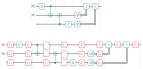
\includegraphics{figures/teleportation_bruit.pdf}
	\end{center}
	\caption{
		Versions idéale (haut) et bruitée (bas) du circuit de téléportation quantique.
	}
	\label{fig:teleportation_bruit}
\end{figure}

Dans un scénario idéal,
un circuit quantique est composé de transformations unitaires,
de préparations d'états, de mesures et de traitements classiques et toutes ces opérations
se font sans erreur.
Par contre,
ce scénario,
bien que très utile pour concevoir des algorithmes quantiques,
est loin de la réalité où chaque opération est imparfaite.
Dans le modèle que je considère pour ce chapitre et les travaux associés,
ces imperfections dans les opérations sont représentées en ajoutant à la suite
de chaque opération parfaite un canal bruité tel qu'illustré à la figure~\ref{fig:teleportation_bruit}.
De plus,
comme les circuits considérés inclus du traitement classique,
il est supposé que les bits sont parfait,
ce qui est assez près de la réalité.

Selon l'opération qui est effectuée,
un canal bruité différent est utilisé.
Dans tous les cas,
la probabilité d'une erreur est $p$.
De plus, 
le circuit est divisé en étapes telles qu'à chacune d'elles,
exactement une opération affecte chaque qubit.
Pour ce faire,
lorsqu'un qubit est inactif,
il est considéré que l'opérateur $I$ est appliqué.
Également,
il n'est pas exclue qu'une opération affecte plusieurs qubits lors de la même étape.

Pour la préparation d'un état propre de $Z$, soit $\ket 0$ ou $\ket 1$,
le canal 
\begin{align}
\mathcal E_X(\rho) = (1 - p)\rho + pX\rho X
\end{align}
est appliqué.
Un canal similaire, $\mathcal E_Z$, est appliqué après la préparation
d'un état propre de $X$.
Ensuite,
le canal
\begin{align}
	\mathcal E_1(\rho) = (1 - p)\rho + \frac{p}{3}(X\rho X + Y\rho Y + Z\rho Z)
\end{align}
est appliqué après une transformation unitaire à un seul qubit.
Dans ce cas,
lorsqu'il y a une erreur,
celle-ci est choisie uniformément entre $X$, $Y$ et $Z$.
De même,
après une transformation unitaire à deux qubits,
le canal
\begin{align}
	\mathcal E_2(\rho)
	= (1 - p)\rho
	+ \frac{p}{15}\sum_{P \in \mathcal P_2^*\setminus \qty{II}} P\rho P
\end{align}
est appliqué,
où $\mathcal P_2^*$ est le groupe de Pauli à 2 qubits sans les phases.
Finalement,
à la suite d'une mesure d'un opérateur de Pauli,
le résultat est renversé avec probabilité $p$.
Cela est équivalent au canal binaire symétrique du premier chapitre
et est noté $\mathcal E_m$.

Le circuit de téléportation illustré à la figure~\ref{fig:teleportation_bruit},
dans sa version idéale et sa version bruité,
constitue dans son ensemble une transformation (non unitaire) à un qubit.
En effet,
bien que celui-ci utilise,
seul le troisième peut avoir un état arbitraire en entrée et un seul qubit reste à la sortie.
L'ensemble des circuits que je considérerai ont cette forme,
c'est-à-dire qu'ils transforment $s$ qubits vers $s$ de manière 
potentiellement non unitaire à l'aide de diverses opérations classiques et quantiques
et de qubits supplémentaires.
Je noterai $N$ le nombre total de qubits du circuit et $\tau$
la profondeur, soit le nombre d'étapes du circuit. 

En raison de l'ajout d'un canal bruité après chaque opération,
il est peu probable que l'état à la sortie du circuit soit l'état désiré.
Pour contrer ce problème,
les états à l'entrée et la sortie du circuit sont encodés dans un code correcteur.
Cela implique par contre de modifier le circuit pour prendre en compte l'encodage des qubits.
Pour évaluer la capacité d'un circuit modifié à tolérer les erreurs,
on vérifie si un décodeur idéal, comme le décodeur de maximum de vraissemblance, est en 
mesure de corriger les erreurs à la sortie du circuit~\cite{gottesman_introduction_2009}.
Ainsi,
pour un circuit $C$,
un état arbitraire $\ket{\psi}$,
sa version encodée $\ket{\bar{\psi}}$ à l'aide d'un code $[n, k]$
et un décodeur optimal $\mathcal D$,
un circuit $T$ est un adaptation tolérante aux fautes de $C$ si,
avec forte probabilité,
\begin{align}
	\mathcal D\qty(T \cdot \mathcal E_1^{n}\qty(\op{\bar \psi}) \cdot T^{\dag})
	= \ket{\bar \phi},
	\label{eq:tol_faute_condition}
\end{align}
où $\ket{\bar \phi}$ est la version encodé de $\ket{\phi} = C \ket\psi$.

Il n'est pas évident qu'il est possible de construire des circuits tolérants aux fautes
puisque l'encodage demande d'utiliser une plus grand nombre de qubits,
ce qui représente un plus grand risque d'erreurs.
Par contre,
le théorème du seuil~\cite{aharonov_fault-tolerant_1999} stipule que si la probabilité d'erreur
par opération $p$ est inférieure à une valeur seuil $p^*$,
alors il est possible de construire un circuit tolérant aux fautes satisfaisant
l'équation~\ref{eq:tol_faute_condition} avec une probabilité arbitrairement près de 1.
La probabilité de seuil mesurée en pratique dépend des codes correcteur utilisés
et des détails d'implémentation du circuit.
Ainsi,
la valeur de se seuil est une métrique importante dans la performance d'un circuit tolérant aux fautes.
En effet,
un seuil élevé permet d'utiliser le circuit avec des systèmes plus bruyant.

Le cas étudié dans les travaux de cette thèse est le cas simple d'une mémoire quantique 
où la version idéale du circuit correspond à l'opérateur identité sur chaque qubit répété à chaque étape.
Bien que ce circuit semble très simple,
il s'agit d'un passage essentiel pour réaliser des circuits plus complexe comme le circuit
de téléportation.
De plus,
lorsque ce circuit est remplacé par sa version bruitée,
chaque qubit à chaque étape est affecté par le canal bruité $\mathcal E_1$.
Ainsi,
si rien n'est fait,
la probabilité d'avoir l'état initial après $t$ étapes pour $k$ qubits est de l'ordre de $p^{kt}$,
c'est-à-dire qu'elle diminue exponentiellement avec $k$ et $t$.

L'astuce pour construire une mémoire quantique tolérante aux fautes
est de constamment faire la correction des erreurs.
Ainsi,
le circuit est remplacé par une succession de mesure du syndrome
et d'application de la correction obtenue par un décodeur.
Bien sur, 
chacune des opérations nécessaires dans les deux cas est suivie d'un canal bruité.

En général,
le décodeur n'est pas optimal puisque cela requiert un temps de calcul beaucoup trop élevé.
Il est plutôt commun de choisir un décodeur sous-optimal,
mais trouvant une correction en temps polynomial.
Dans ce cas,
on suppose que le temps de décodage est nul 
et qu'aucune erreur ne peut apparaitre durant lors du décodage.

Dans le cadre de cette thèse,
je ne m'intéresse pas aux décodeurs et je me contente des algorithmes de décodage standards.
Cela me permet de me concenter sur les circuits de mesure du syndrome.
Dans le cas idéal,
un circuit de mesure du syndrome prend en entrée un état arbitraire
et retourne ce même état en plus d'une séquence de bits correspondant au syndrome de l'état.

Les mesures du syndrome se font à l'aide d'opérations appartenant au groupe de Clifford,
de préparation des états propres de $X$ et $Z$ et de la mesure de ces opérateurs
pour un seul qubit.
Le groupe de Clifford est l'ensemble des transformations unitaires $U$ telles que,
pour tous opérateurs de Pauli $P \in \mathcal P$,
il existe un $Q \in \mathcal P$ pour lequel $PU = UQ$.
Comme les erreurs sont décomposées sur la base des opérateurs de Pauli,
il est possible de remplacer une erreur appliquée avant un opérateur de Clifford
par une erreur appliquée après.
Cela permet ainsi de remplacer toutes les erreurs effectant un circuit composé d'opérateurs de Clifford, p
par une seule erreur à la fin du circuit.

Le groupe de Clifford est généré par l'opérateur d'Hadamard $H$,
l'opérateur de phase $S$ et l'opérateur de non-contrôlé $\text{CNOT}$
et inclus, entre autres, les opérateurs de Pauli.
Parmi ceux-ci,
la porte $\text{CNOT}$,
inversant le deuxième qubit si le premier est dans l'état $\ket{1}$,
est l'unique opérateur utilisé pour la construction des circuits de mesure du syndrome 
présentés dans l'article.
L'action de CNOT est 
\begin{align}
	\text{CNOT} = \op{00}{00} + \op{01}{01} + \op{10}{11} + \op{11}{10}
\end{align}
et l'on vérifie facilement que
\begin{align}
	&XI \cdot \text{CNOT} = \text{CNOT} \cdot XX,
	&&ZI \cdot \text{CNOT} = \text{CNOT} \cdot ZI, \notag \\
	&IX \cdot \text{CNOT} = \text{CNOT} \cdot IX,
	&&IZ \cdot \text{CNOT} = \text{CNOT} \cdot ZZ,
	\label{eq:cnot_pauli}
\end{align}
les autres relations étant générées à partir de ces dernières.

\begin{figure}
	\centering
	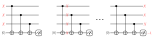
\includegraphics{figures/mesure_syndrome.pdf}
	\caption[Exemple de mesure de syndrome]{
		Propagation d'erreurs de type $X$ dans le circuit de mesure d'un
		stabilisateur de type $Z$ supporté sur trois qubits.
		L'erreur initiale, la conjugaison avec le premier CNOT 
		et l'état final en supposant un circuit idéal sont illustrés.
	}
	\label{fig:mesure_syndrome}
\end{figure}

Pour mesurer la parité d'un générateur du groupe stabilisateur de type $Z$,
un qubit supplémentaire, nommé qubit de mesure,
est d'abord préparé dans l'état $\ket 0$.
Ensuite,
une opération CNOT est faite à partir de chacun des qubits supportant de stabilisateur
vers le qubit de mesure.
Finalement,
ce qubit est mesuré dans la base de l'opérateur $Z$.
Tel que mentionnée à l'équation~\ref{eq:cnot_pauli},
une erreur $X$ affectant le premier qubit du CNOT est remplacée
par une erreur $X$ sur ce même qubit et sur le qubit de mesure.
Dans le cas contraire,
une erreur $X$ sur le qubit de mesure ne se propage sur l'autre qubit 
impliqué dans le CNOT.
Ainsi,
comme illustré à la figure~\ref{fig:mesure_syndrome},
après l'application des portes CNOT,
le qubit de mesure se retrouve dans l'état $X^r\ket{0}$ où 
$r$ et le nombre de qubits affecté par une erreur $X$ à l'entrée du circuit.
Une mesure dans la base $Z$ permet donc de mesurer la parité de $r$.
Comme les erreurs $Z$ n'ont aucun impact sur la valeur de la mesure,
cela complète le circuit.

Pour mesurer la parité d'un stabilisateur de type $X$,
un circuit similaire est utilisé.
Dans celui-ci,
le qubit de mesure est préparé dans l'état $\ket +$ au lieu de l'état $\ket 0$,
la direction des portes CNOT est inversée
et la mesure ce fait dans la base de l'opérateur $X$.
Encore une fois,
il est possible de valider ce circuit avec les relations de l'équation~\ref{eq:cnot_pauli}.

Le circuit pour mesurer la totalité du syndrome est obtenue 
en chainant les circuits pour mesurer la parité de chacun des
générateurs du groupe stabilisateur.
De prime abord,
cette approche à deux problèmes majeurs.
Premièrement,
la profondeur du circuit total augmente linéairement avec le nombre 
de générateurs.
Deuxièmement,
en cas d'erreurs dans les circuits individuels,
la valeur du syndrome peut ne pas correspondre à l'erreur sur le système.

Les travaux de ce chapitre addressent c'est deux problèmes.
D'abord,
il est montré qu'il est possible d'effectuer des mesures de syndromes en parallèle
pour tout codes CSS.
Cela permet de réduire la profondeur du circuit à une constante qui ne dépend que
du degré du graphe de Tanner,
soit le nombre d'arête du sommet avec le plus de connexions.
Ensuite,
des simulations numériques ont montré que même avec cette approche simple
de mesure du syndrome,
le seuil de tolérance aux fautes obtenus avec les codes de produits d'hypergraphe
est du même ordre de grandeur que les meilleurs seuils connus.
Ainsi,
remplacer les circuits de mesure de chaque générateur par des circuits
naturellement plus tolérant aux fautes ne peut qu'améliorer les résultats qui seront présentés.
Il s'agit d'ailleurs d'un avenue intéressante pour de futurs travaux de recherche.

Dans la prochaine section,
je vais introduire les codes de produits d'hypergraphes, 
la famille de codes LDPC qui a été étudiée plus en détails dans l'article.

\section{Codes de produits d'hypergraphes et codes expanseurs}

\section{Article}

\includepdf[pages=-]{articles/planar_layout.pdf}

